\documentclass{standalone}
\usepackage{tikz}
\usepackage{hsbcommon}
    \begin{document}
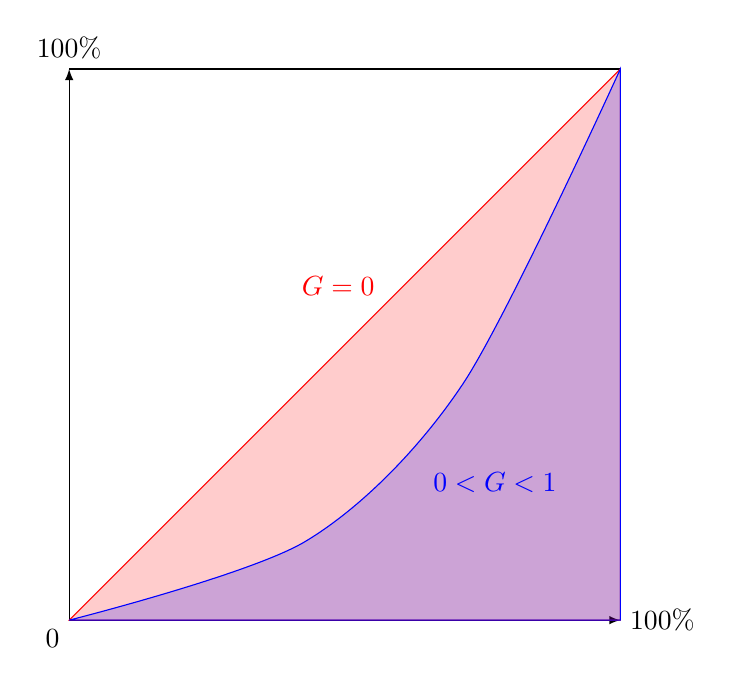
\begin{tikzpicture}
        \draw[->,>=latex] (0,0) node[below left] {$0$} -- (0,7) node [above] {$100\%$};
        \draw[->,>=latex] (0,0) -- (7,0) node [right] {$100\%$};
        \draw (0,7) -- (7,7) -- (7,0);

        \draw[color=red,fill=red,fill opacity=0.2] (0,0) -- (7,7) -- (7,0) -- cycle;

        \node[red, above left] at (4,4) {$G=0$};

        
        \draw[color=blue, fill=blue,fill opacity=0.2,smooth] plot coordinates {(0,0) (3,1) (5,3) (7,7)}  -- (7,0)  -- (0,0) ;
        
        \node[blue, below right] at (4.5,2) {$0<G<1$};
        
    \end{tikzpicture}
\end{document}
